\part{Introduction}

\paragraph{}
Every day millions of people find themselves in the troublesome task of 
computing a route to their desired destination. We'll provide directions for 
their journey with state of the art routing algorithms in a safe way. The 
service will provide the following transportation modes when querying a route: 
car, foot and bicycle.

\paragraph{Problem}
Navigating a city like London is a complicated matter even during normal times, 
let alone during rush hour. Due to the convoluted nature of London’s road 
network accidents and disruptions are common occurrences that afflict all road 
users during their journeys.

\paragraph{Objective}
We’ll provide analytic functionalities to find hotspots in the road network 
graph, that is to collect information about all users' journeys and visualize 
the most congested routes/graph’s regions.

\begin{figure}[H]
	\centering
	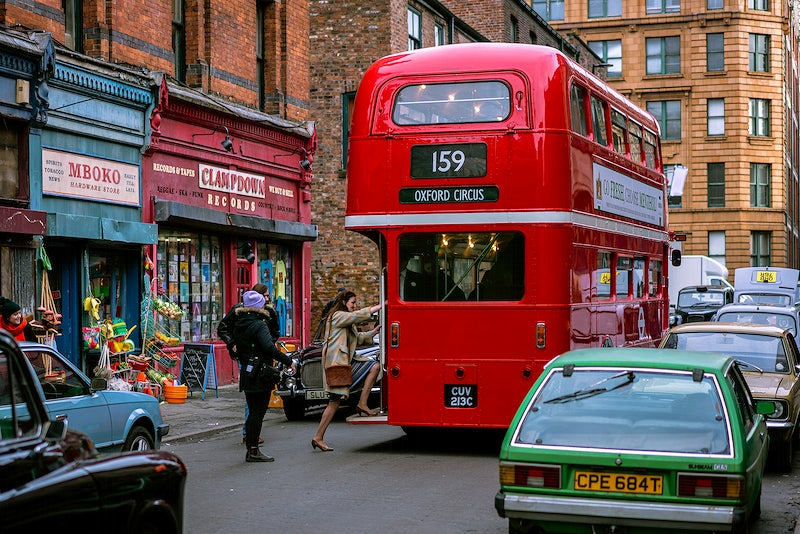
\includegraphics[width=0.9\linewidth]{assets/londontraffic.jpg}
\end{figure}

\paragraph{Source Code}
The source code for the final application, as said in the next chapters 
\ref{banana} can be found at the following link: 
\url{https://github.com/scarburato/LargeScaleDBsProject}, in particular the 
Java application is found under 
\href{https://github.com/scarburato/LargeScaleDBsProject/tree/master/src/libCommon}
{\texttt{libCommon}}
and the neo4j procedure under 
\href{https://github.com/scarburato/neo4jpoormensAstar/tree/9cdfe3be44639d788bac4bfa2f8371f6826b828c}
{\texttt{routingNeo4jProcedure}}.


